\addcontentsline{toc}{chapter}{Introduction}
\chapter*{Introduction}

\addcontentsline{toc}{section}{What is the subject of the internship ?}
\section*{What is the subject of the internship ?}

This internship aims to use reinforcement learning to optimize epidemic crisis management. This therefore includes designing the environment for the epidemic spread and applying reinforcement learning to its assessments. This optimization is multi-criteria since it aims to dissipate or limit infectious exchanges while stabilizing the economy of the territory studied.\\

This project focuses on Luxembourg society and is coded in Python language since there are many libraries already interesting for the development of the program.\\

For the sake of perfectionism, the development of the environment has taken time and many elements still remain to be implemented in the program. It was necessary to imagine everything without a guide, integrating the SumoMobility tool, to have a realistic design, efficient and that can be adapted as and when needs and perspectives of evolution.\\

At the end of this internship, only a simple part of the environment is implemented. It would be necessary to have more time to make the environment more complex/realistic, adapt the simulated results with those of the real data, be able to determine actions of societal control and finally optimize these decisions according to several criteria and constraints.\\

The idea is to think step by step, perfect and make the environment more and more realistic with design testing. This is the very basis of optimization so it is the most essential !

\newpage

\addcontentsline{toc}{section}{A quick tour on the environment}
\section*{A quick tour on the environment}

The focus here is on epidemics that are transmitted by air. The design of the environment for this project is poorly adapted to other means of transmission such as sexually transmitted diseases such as AIDS.\\

The spread of infectious agents in society cannot be predicted a priori. It is necessary to wait for the transformation of the environment to characterize the parameters of an epidemic. An epidemic is identified only after discovering infected cases in society and making the link with the emergence of a new epidemic. The evolution of an airborne epidemic extends geographically in a rather chaotic way, with the dynamic entropy of carrier individuals in society. To model this environment, it is necessary to break down society by individuals and spaces/places of passage. Each individual circulates in society through different spaces in his daily life. Infectious exchanges take place with the proximity of healthy and carrier individuals.\\

Several scales can be distinguished in the representation of the environment. Very locally, it is too absurd to represent the spread of infectious agents within an individual's organism, especially considering the complexity and diversity of organisms. But we will see that we can have a very simplistic approach to the infectious functioning of an organism by considering the duality between antigens and antibodies. At the scale of a confined or semi-enclosed space, it is quite accessible to represent the infectious exchanges between individuals. Then, more generally, there are two scales that can be dissociated at the regional level and then at the national level.\\

With a view to societal optimization, this project centralizes its approach on a regional scale. We take a specific territory containing several spaces and synthesize the infectious exchanges in these different spaces. In a more developed version, the project can be extended to multi-territorial or national representation, where decisions may be different depending on the region. In parallel, we will also be interested in the mobility of individuals within the architecture of spaces. The outlook for developments is discussed in more detail at the end of this report.\\

\addcontentsline{toc}{section}{What main tools are used ?}
\section*{What main tools are used ?}

The starting point of the program is the description of a territory by an openstreetmap file that makes it possible to obtain the spaces of interest of a region as well as the tracks for the circulation of individuals. The description of these files is done by contributors and is relatively well detailed. It should be noted that the veracity of the data described or their updating are sometimes questionable. In our use for rich and popular parts of the world like Luxembourg, the files are far more than enough.\\

The second tool is SumoMobility, which is an implementation dedicated to civil engineering to digitize urban traffic with several distinct types of transport. The program can directly use an openstreepmap file of the input region to get the road network. It is a very complex and interesting tool to reproduce the mobility of a society. However, one of the difficulties is that it is very much oriented around trafficking and not individuals. It is therefore necessary to adapt our implementation. This tool has the advantage of being popular and can provide sufficient complexity to our program with the mobility and traffic constraints of the company. It should also be noted that there are research studies on traffic demands and traffic statistics that may be interesting to deepen the project. One example is Luxembourg Sumo Traffic Scenario (LuST) produced by Laura Codeca, Raphael Frank and Thomas Engel, from the University of Luxembourg.\\

These tools will be more detailed as the report progresses.\\

Similarly, we can note the use of a pre-existing library in Python for reinforcement learning called rlib. This implementation is very complete but will not be developed in this report due to lack of time. Of course, the project uses other standard Python libraries that are not like real tools.\\

\newpage

\addcontentsline{toc}{section}{Sophisticated approach}
\section*{Sophisticated approach}

Before talking about multicriteria optimization, it is necessary to work on the design of the environment in detail. This is the basis of the project : the more the environment is perfected, the more applicable and realistic its optimization will be. It is from this point of view that my internship focused on the development of the environment. For the sake of perfectionism, it is essential to think carefully about the interlocking designs/ideas to be able to break down the implementation and anticipate its use for related topics or to foresee prospects for evolution.\\

As a result, there are five main layers in the environment : individuals, spaces, mobility, infectious agents and combinatorial decisions. Each of them will be detailed in the following parts.\\

In detail, we use cartographic and demographic data to initialize the territory we are studying. This phase is essential and it is absurd to determine an optimization on a little-known environment. This is why we will talk more about "digitalization" than simulation. More precisely, this phase will be called the static digitalization of society, which brings together individuals and spaces.\\

Secondly, we are concerned with the dynamic digitalization of individuals in different spaces. It is a complex phase. This is where we can find a parallel with a neural network. From an initial environment composed of individuals and spaces, it must be possible to evaluate the dynamics of society over a large set of days, each with different characteristics. It is like a black box where we find the individuals and spaces at the entrance, and the detailed occupations of the spaces at the exit.\\

So why not simply use a neural network to predict the dynamics of society ?\\

The very concept of a neuron is to assimilate several data, process them and summarize them into simple information. It's not intuitive about developing a complete dynamic assessment for each individual and each space. So a priori we could summarize mobility and be satisfied with more or less simple statistics. We can find the usefulness of a neural network which is to solve a goal of classification or prediction of a set of data without context. But if we manage to approach the reality of society and observe a real dynamic digitalization, we can have much more relevant and unmodified information. Our data processing is much more precise and leaves very little room for error. You don't make a pastry recipe by playing dice! This is the complex part of any project which is to work on the details of things. When done well, there is only a tiny uncertainty about the final result. With a view to multi-criteria optimization of evaluations, details about the environment are therefore more than essential.\\

To the question how to make dynamic digitalization reliable and realistic ?\\

This is the problem, and the challenge of environmental design. The part concerning the mobility of individuals in spaces and dealt with later in the report. We will see that we can find a form of training of this digitalization as we find in a neural network. Of course, this training is not mandatory here since we can already reproduce a totally random mobility and obtain a dynamic of individuals. This is also the current result of the internship but it must be taken into account that it is absurd. But this at least has the merit of representing the potential of this project.\\

The training could be carried out with traffic demands, observed data on the affluence of places for example. We may be interested in tracing individuals via network coverage but this poses ethical problems for the individual. As a reminder, the interest here is not to spy on or manipulate individuals via their personal data ; The project focuses on predicting the movements of a territory to optimize health risks and maximize economic stability. It must be benevolent for individuals and the population in general.\\

From there, it is interesting to dissociate digitalization from society and infectious spread. For benevolent side projects or even to simplify the maintenance of the implementation, it is interesting to be able to digitize a territory independently of an epidemic consideration.\\

The layer concerning infectious agents is an addition of digitalization. Of course, it brings specific characteristics to individuals, spaces and mobility. The interest is not to make these parameters blocking for a simple societal digitalization. It will be seen that we can also train the parameters of each infectious agent with observed data. However, as noted above, the parameters of an infectious agent can only be characterized retrospectively. The whole point is to perfect this adaptation with historical data such as Covid-19. It is by training that you become an expert !\\

The ideal of this project is to propose as quickly and as appropriately as possible an optimal decision sequence for society, producing a realistic and benevolent territorial digitalization towards the individual.\\

It is clear, however, that the relevance of the use of observed infectious data is highly dependent on the use of society's dynamic data. One cannot properly approach the reality of an epidemic spread without having a robust and stable basis for the dynamic behaviour of a society.\\

So what are combinatorial decisions based on ?\\

Such an environment cannot be optimized by leaving a large research space. It is necessary to define a predefined number of decisions, with their detailed constraints in the environment. These decisions impact the dynamic digitalization of society and modify the mobility of society. There are differences in the sequence of spaces traversed by each individual as well as in the affluence of these spaces. It is from this data that evaluation scores on several different criteria are established. These scores form the support of multi-criteria combinatorial optimization that establishes the most appropriate sequence of decisions possible.\\

Combinatorial decisions thus form a final layer of the program and are not essential for simple societal digitalization. One of the problems is therefore to code the static and dynamic digitalization of society, while leaving a possible modification on the part of a higher layer.\\

\newpage

\addcontentsline{toc}{section}{Why invest in this project ?}
\section*{Why invest in this project ?}

Simplistic simulations can already be used to predict the health evolution of an epidemic. For example, the experience presented with the CRS model in thefollowing presentation includes : \href{https://www.youtube.com/watch?v=gxAaO2rsdIs}{\textit{Youtube Example}}\\

With this project, we propose to bring a real approach to society : \\we want to consider the places of passage specific to each individual, predict societal behaviors and study infectious exchanges according to different parameters. In a defined region, real data such as map, demographic, epidemic and many other data is used. The objective of this project is to have a multi-criteria optimization perspective of epidemic management. We want to act with kindness towards the individual, limit health risks and maximize the economic stability of a territory. We define this territory on Luxembourg, and more precisely on the Belval campus in Esch-sur-Alzette for this internship. But this project is intended to adapt to any territory.\\

\begin{figure}[h]
  \centering
  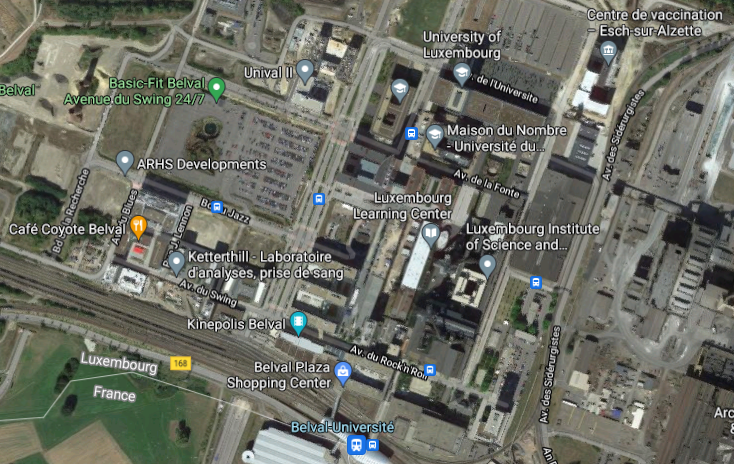
\includegraphics[width=0.8\linewidth]{Media/BelvalMaps.png}
  \caption{\centering {\small A satellite view of the Belval campus in Esch-sur-Alzette from Google Maps.}}
  \label{fig:belvalmaps}
\end{figure}

To talk in depth about the motivations of such a project, it is more than necessary to talk about moral principles and human benevolence, especially when talking about artificial intelligence. We go beyond the technical framework of an engineering internship but it is interesting to talk about it in the appendix at the end of this report. \\

Historically, natural, environmental and epidemic disasters can be classified as the largest humanitarian disasters. What other problems are more essential to optimize ? We do not count wars since there is a voluntary desire on the part of man to destroy his neighbor, which must not be optimized in the ethical sense. The stakes of humanitarian disasters are the most important in the world, whether human, economic, psychological, etc. At these levels, the slightest optimizations at the lowest scales are always crucial.\\

In our case here of epidemic crises, the subject is topical with Covid-19. Current events show us all the importance of optimizing the management of an epidemic crisis. From a historical point of view, no technology at the time of the old crises made it possible to design an optimization of decisions. Remembering the appalling damage of previous health crises, it seems obvious that they must prepare as well as possible to optimize future epidemics/pandemics. In the immediate term, this would also support current decisions in the management of Covid-19.\\

As mentioned earlier, by breaking down the elements of this project, one can also find other interests such as the modeling of a society and its dynamics, independently of a spread of infectious agents. In addition, beyond the novelties in the digitalization of an epidemic, we also find an interest in optimizing several criteria in epidemic management : it will be interesting to think about looking for other avenues of multi-criteria optimization with reinforcement learning, which are not already addressed in research. These avenues of exploitation may include the complex environment and the possibility of accurately describing actions in the environment. With this project, it is also possible to detail many evaluations with very different criteria.\\